\chapter{\IfLanguageName{dutch}{Resultaten}{Results}}%
\label{ch:resultaten}

In dit hoofdstuk worden de resultaten van de route generatie besproken. 
Volgende routes worden gegenereerd:
\begin{itemize}
    \item 5 km route
    \item 10 km route
    \item 50 km route
    \item 100 km route
\end{itemize}
\section{Zonder geavanceerde opties}

\subsection{5 km route}

\begin{figure}[H]
    \centering
    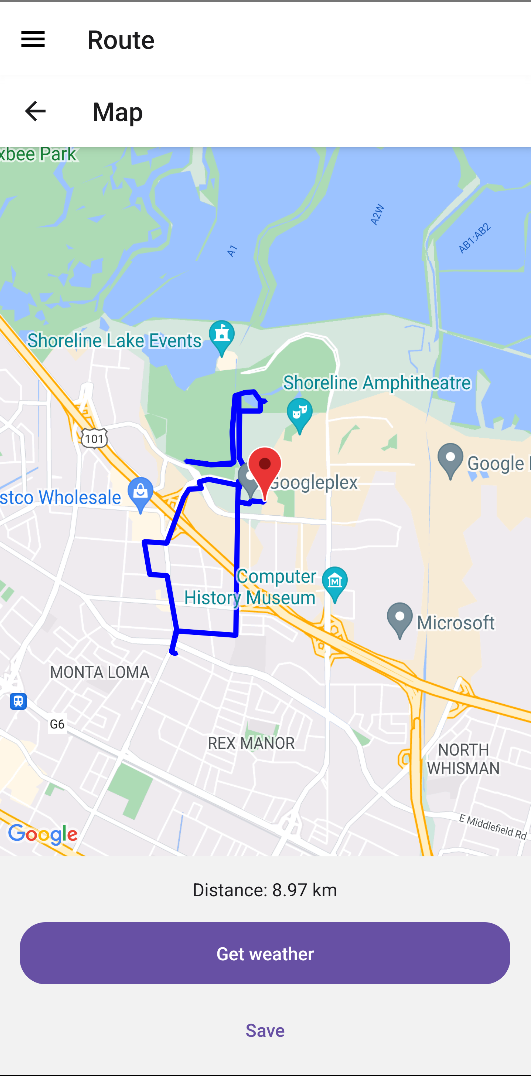
\includegraphics[width=20em]{5km_route}
    \caption{5 km route}
    \label{fig:5km_route}

\end{figure}

De gegenereerde route is 8.97 km lang, dit is langer dan de gevraagde 5 km. Dit komt omdat de route steeds elk punt van de route probeert te verbinden met de kortste afstand. Dit kan lijden tot een langere route dan gevraagd.
De vorm van de route is vooral een lus, maar er zijn ook enkele stukken die heen en terug gaan.

Uitgedruk in procent is de route 79.4\% langer dan gevraagd.
\subsection{10 km route}

\begin{figure}[H]
    \centering
    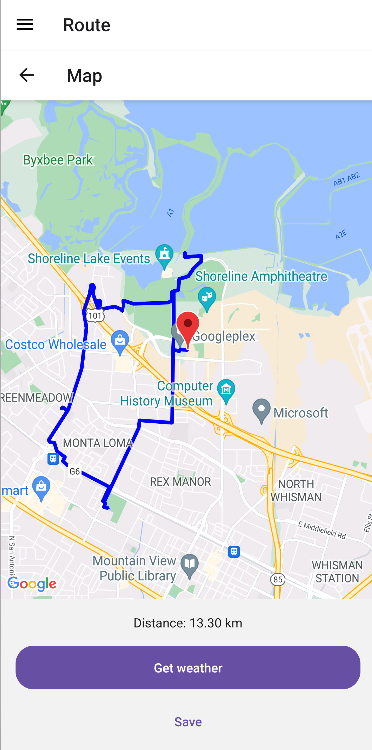
\includegraphics[width=20em]{10km_route}
    \caption{10 km route}
    \label{fig:10km_route}

\end{figure}

De gegenereerde route is 13.30 km lang, dit is langer dan de gevraagde 10 km. De vorm van de route lijkt al meer op een volledige lustructuur, maar er zijn nog steeds enkele stukken die heen en terug gaan.

Uitgedruk in procent is de route 33\% langer dan gevraagd.

\subsection{50 km route}

\begin{figure}[H]
    \centering
    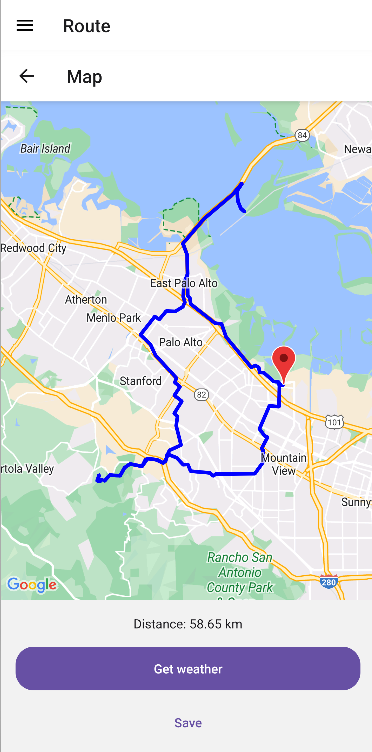
\includegraphics[width=20em]{50km_route}
    \caption{50 km route}
    \label{fig:50km_route}

\end{figure}

De gegenereerde route is 58.65 km lang, dit is ook langer dan gevraagd. De vorm van de route is een volledige lus, met 2 'takken' die hieruit springen, die heen en terug gaan.

Uitgedruk in procent is de route 17.3\% langer dan gevraagd.

\subsection{100 km route}

\begin{figure}[H]
    \centering
    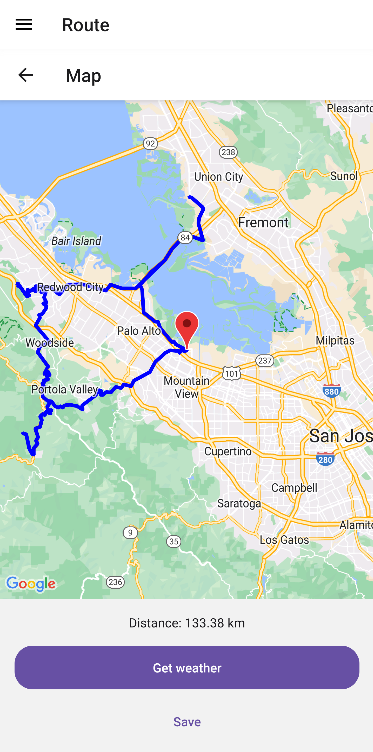
\includegraphics[width=20em]{100km_route}
    \caption{100 km route}
    \label{fig:100km_route}

\end{figure}

De gegenereerde route is 133.38km lang, dit is langer dan gevraagd. Ook hier is de vorm van de route een volledige lus, met nu 3 'takken' die hieruit springen, die heen en terug gaan.

Uitgedruk in procent is de route 33.4\% langer dan gevraagd.

\pagebreak

\subsection{Algemeen}

De routes die gegenereerd worden zonder geavanceerde opties zijn de meest eenvoudige routes. De routes zijn vooral lussen, met enkele stukken die heen en terug gaan. De routes zijn vaak langer dan gevraagd.

Gemiddeld is de route 40.8\% langer dan gevraagd.

\section{Met geavanceerde opties}

Als geavanceerde opties worden de volgende opties ingesteld:
\begin{itemize}
    \item Elevation: Medium
    \item Underground: ground
    \item Points of interest: park, running, path, footway, tree, viewpoint
\end{itemize}

\subsection{5 km route}

\begin{figure}[H]
    \centering
    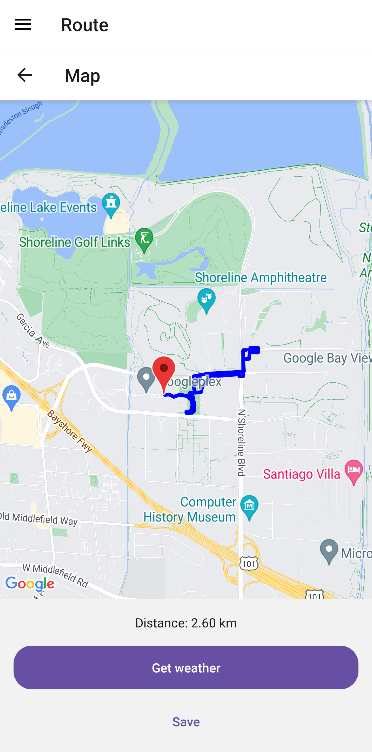
\includegraphics[width=20em]{5km_route_geavanceerd}
    \caption{5 km route met geavanceerde opties}
    \label{fig:5km_route_geavanceerd}

\end{figure}

De gegenereerde route is 2.60 km lang, dit is bijna de helft van de gevraagde 5km. De vorm van de route bestaat enkel uit stukken die heen en terug gaan.

Uitgedruk in procent is de route 48\% korter dan gevraagd.

\subsection{10 km route}

\begin{figure}[H]
    \centering
    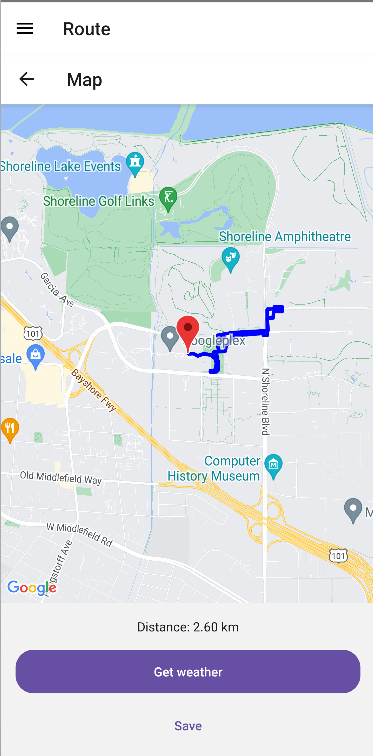
\includegraphics[width=20em]{10km_route_geavanceerd}
    \caption{10 km route met geavanceerde opties}
    \label{fig:10km_route_geavanceerd}

\end{figure}

De gegenereerde route is 2.60 km lang, dit is veel korter dan de gevraagde 10km. De route lijkt dezelfde te zijn als bij 5km.

Uitgedruk in procent is de route 74\% korter dan gevraagd.

\subsection{50 km route}

\begin{figure}[H]
    \centering
    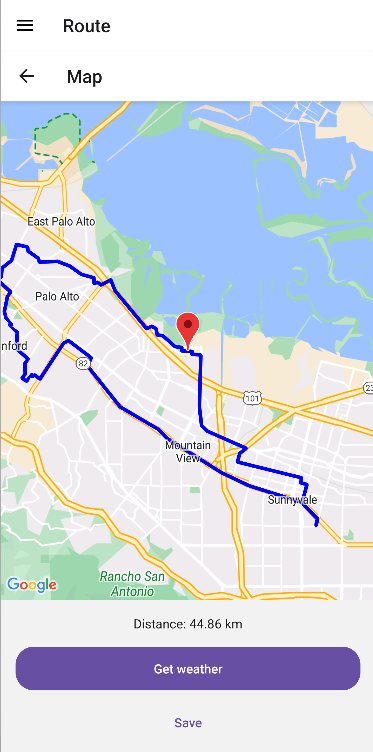
\includegraphics[width=20em]{50km_route_geavanceerd}
    \caption{50 km route met geavanceerde opties}
    \label{fig:50km_route_geavanceerd}

\end{figure}

De gegenereerde route is 44.86 km lang, dit is een beetje korter dan de gevraagde 50km. Deze route is een volledige lus.

Uitgedruk in procent is de route 10.28\% korter dan gevraagd.

\subsection{100 km route}

\begin{figure}[H]
    \centering
    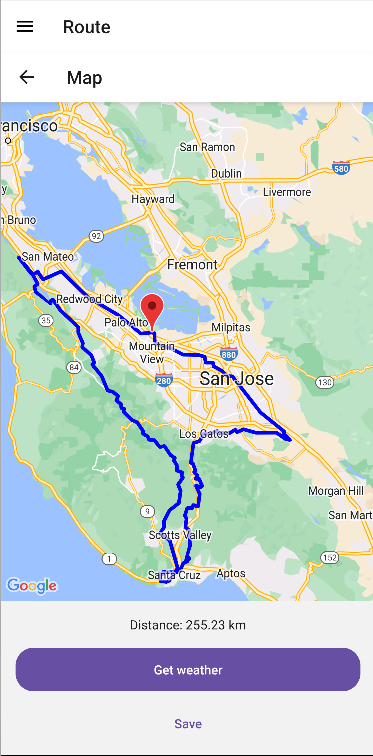
\includegraphics[width=20em]{100km_route_geavanceerd}
    \caption{100 km route met geavanceerde opties}
    \label{fig:100km_route_geavanceerd}
\end{figure}

De gegenereerde route is 255.23 km lang, dit is enorm veel langer dan de gevraagde 100 km. Deze route lijkt echter wel een volledige lus te zijn.

Uitgedruk in procent is de route 155.23\% langer dan gevraagd.


\pagebreak

\subsection{Algemeen}

De routes die gegenereerd worden met geavanceerde opties zijn doorgaans korter dan de gevraagde afstand. Met uitzondering de route van 100 km, deze is veel langer dan gevraagd.
De routes bestaan meer uit lussen. De variatie in afstand tussen de routes ligt aan de punten die de OverPass API teruggeeft en is sterk afhankelijk van de locatie van de gebruiker.

Gemiddeld is de route 41.4\% korter dan gevraagd.

\section{Met zelf gekozen punten}

Als zelf gekozen punten worden de volgende punten ingesteld:
\begin{itemize}
    \item Start: HOGENT campus Schoonmeersen, Valentin Vaerwyckweg, Ghent, Belgium
    \item Einde: Overpoortstraat, Ghent, Belgium
    \item Punt: Gravensteen, Sint-Veerleplein, Ghent, Belgium
\end{itemize}

De geavanceerde opties worden behouden van vorige sectie.

\subsection{5 km route}

\begin{figure}[H]
    \centering
    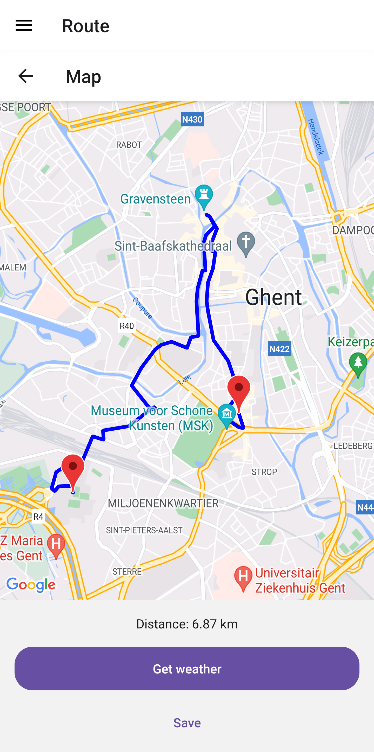
\includegraphics[width=20em]{5km_route_zelf}
    \caption{5 km route met zelf gekozen punten}
    \label{fig:5km_route_zelf}

\end{figure}

De gegenereerde route is 6.87 km lang, dit is een beetje langer dan de gevraagde 5 km.

Uitgedruk in procent is de route 37.4\% langer dan gevraagd

\subsection{10 km route}

\begin{figure}[H]
    \centering
    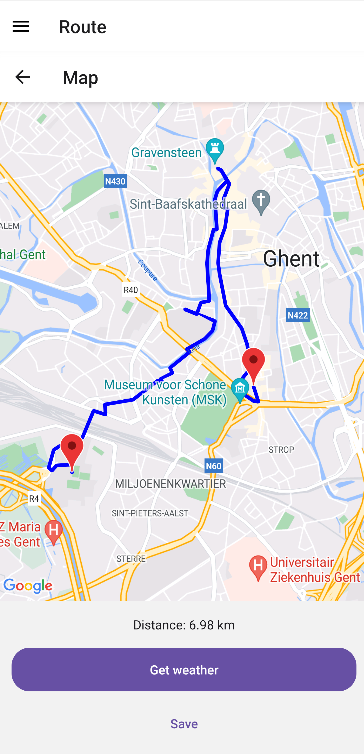
\includegraphics[width=20em]{10km_route_zelf}
    \caption{10 km route met zelf gekozen punten}
    \label{fig:10km_route_zelf}

\end{figure}

De gegenereerde route is 6.98 km lang, dit is korter dan de gevraagde 10 km en is bijna hetzelfde als de 5 km route.

Uitgedruk in procent is de route 30.2\% korter dan gevraagd.

\subsection{50 km route}

\begin{figure}[H]
    \centering
    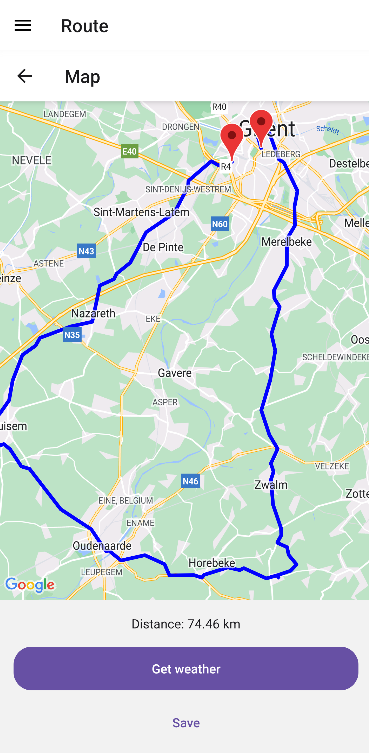
\includegraphics[width=20em]{50km_route_zelf}
    \caption{50 km route met zelf gekozen punten}
    \label{fig:50km_route_zelf}

\end{figure}

De gegenereerde route is 74.46 km lang, dit is langer dan de gevraagde 50 km.

Uitgedruk in procent is de route 48.9\% langer dan gevraagd.

\subsection{100 km route}

\begin{figure}[H]
    \centering
    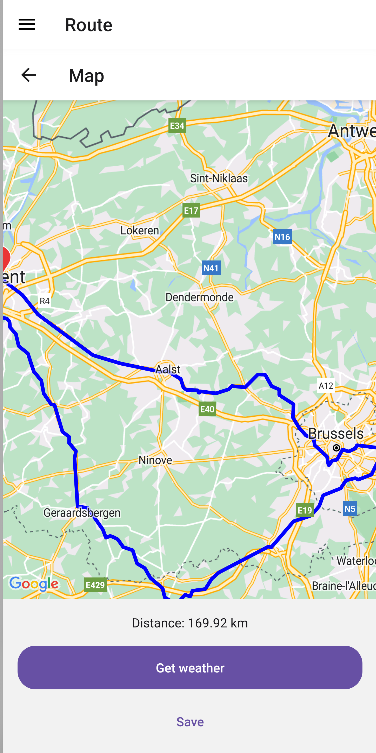
\includegraphics[width=20em]{100km_route_zelf}
    \caption{100 km route met zelf gekozen punten}
    \label{fig:100km_route_zelf}

\end{figure}

De gegenereerde route is 169.92 km lang, dit is langer dan de gevraagde 100 km.

Uitgedruk in procent is de route 69.92\% langer dan gevraagd


\pagebreak

\subsection{Algemeen}

De routes die gegenereerd worden met zelf gekozen punten zijn doorgaans langer dan de gevraagde afstand. De variatie in afstand tussen de routes ligt aan de punten die de OverPass API teruggeeft en is sterk afhankelijk van de locatie van de gebruiker.

Gemiddeld is de route 46.6\% langer dan gevraagd.

\section{Besluit}

De routes die gegenereerd worden zonder geavanceerde opties zijn de meest eenvoudige routes. De routes zijn vooral lussen, met enkele stukken die heen en terug gaan. De routes zijn ook langer dan gevraagd.
Doorgaans zullen routes die berekent worden op deze manier het minst variabel zijn.

\vspace{1cm}


De routes die gegenereerd worden met geavanceerde opties zijn doorgaans korter dan de gevraagde afstand. Met uitzondering de route van 100 km, deze is veel langer dan gevraagd.
De routes bestaan meer uit lussen. De variatie in afstand tussen de routes ligt aan de punten die de OverPass API teruggeeft en is sterk afhankelijk van de locatie van de gebruiker.
Er werd een poging gedaan om de lengte van de route te beperken in het algoritme, maar deze is niet altijd succesvol. Dit komt omdat de afstand tussen punten in het algoritme in vogelvlucht wordt berekend en niet over de weg.
De kwaliteit van deze routes is sterk afhankelijk van de geavanceerde opties die de gebruiker kiest en de locatie van de gebruiker.

\vspace{1cm}


De routes die gegenereerd worden met zelf gekozen punten zijn doorgaans langer dan de gevraagde afstand. 
De variatie in afstand tussen de routes ligt hier ook aan de punten die de OverPass API teruggeeft en is sterk afhankelijk van de locatie van de gebruiker. 
Het is echter minder extreem en de genereerde routes lijken van betere kwaliteit te zijn dan de routes die gegenereerd worden met geavanceerde opties, zonder zelf gedefinieerde punten.

\vspace{1cm}


Het is steeds mogelijk om op de terug te knop te drukken en een nieuwe route te genereren, de parameters die ingesteld zijn blijven behouden. Dit kan handig zijn als de gebruiker niet tevreden is met de gegenereerde route.







